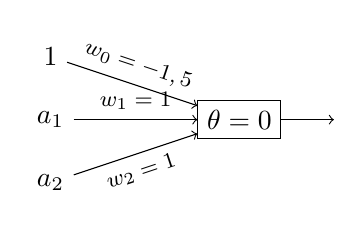
\begin{tikzpicture}[scale=0.4]
	\draw node (w1) {$a_1$} ++(6,0) node[draw] (centro) {$\theta=0$};
	\path (w1) -- ++(0, 2) node (w0) {$1$};
	\path (w1) -- ++(0, -2) node (w2) {$a_2$};
	%\node[init] (centro) {Centro};
	%\node[init, left of=centro] (w1) {$w1$};
	%\node[init] (s2) {$w2$};

	\draw[->] (w1) -- (centro) node[midway,above,sloped] {\footnotesize{$w_1=1$}};
	\draw[->] (w2) -- (centro) node[midway,below,sloped] {\footnotesize{$w_2=1$}};
	\draw[->] (w0) -- (centro) node[midway,above,sloped] {\footnotesize{$w_0=-1,5$}};
	\draw[->] (centro) -- ++(3,0);
\end{tikzpicture}
